\todo{Use a table?}
\todo{Write things specifically for my report? Body frame orientation and so on}
\todo{Add to abbrev}

\section{ECI}
    The Earth-centered inertial (ECI) frame has its origin at the center of the Earth and z-axis intersecting the geographic North Pole. It is denoted by \{i\}.
    

\section{ECEF}
    The Earth-centered, Earth-fixed (ECEF) frame is another coordinate system with origin at the center of mass of the Earth. Its z-axis is also shared with the ECI reference frame, but the x- and y-axes intersects fixed point on the surface of the earth, meaning that it rotates with the Earth about the z-axis. As such, ECEF is not an inertial frame, but for slow moving craft it may be considered as such \cite{fossen2011handbook}. In this thesis, the ECEF frame of reference is denoted by \{e\}. 
    
    \begin{figure}
        \centering
        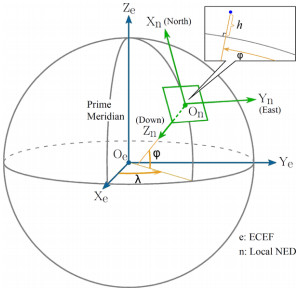
\includegraphics[scale=1]{Appendices/bilder/ECEF_ENU_BETTER.png}
        \caption{NED and ECEF frames}
        \label{fig:ecef-enu}
        \todo{find better figure?}
    \end{figure}
    
\section{NED}
    The north-east-down frame is a location dependent system tangential to the surface of the Earth. The z-axis points down, along the normal of the Earth ellipsoid, while x- and y-axes points north and east, respectively. The NED frame is denoted \{n\}.

\section{Body}
    The body-fixed reference frame is a moving coordinate system fixed to some craft. Both origin and orientation of the coordinate system is chosen freely \todo{And has in this thesis been set to..}. The body system is denoted \{b\}